%mod2-1chapter 1 pages 1-20
\chapter{The Basics of Logical Analysis}

\subsection{What Is Logic?}
In Logic, the object of study is reasoning. This is an activity that humans engage in--when we
make claims and back them up with reasons, or when we make inferences about what follows from
a set of statements.

Like many human activities, reasoning can be done well, or it can be done badly. The goal of logic
is to distinguish good reasoning from bad. Good reasoning is not necessarily effective reasoning;
in fact, as we shall see, bad reasoning is pervasive and often extremely effective--in the sense that
people are often persuaded by it. In Logic, the standard of goodness is not effectiveness in the
sense of persuasiveness, but rather correctness according to logical rules.

In logic, we study the rules and techniques that allow us to distinguish good, correct reasoning
from bad, incorrect reasoning.

Since there is a variety of different types of reasoning, since it's possible to develop various
methods for evaluating each of those types, and since there are different views on what constitutes
correct reasoning, there are many approaches to the logical enterprise. We talk of logic, but also
of logics. A logic is just a set of rules and techniques for distinguishing good reasoning from bad.

So, the object of study in logic is human reasoning, with the goal of distinguishing the good from 
the bad. It is important to note that this approach sets logic apart from an alternative way of 
studying human reasoning, one more proper to a different discipline: psychology. It is possible to 
study human reasoning in a merely descriptive mode: to identify common patterns of reasoning and 
explore their psychological causes, for example. This is not logic. Logic takes up reasoning in a 
prescriptive mode: it tells how we ought to reason, not merely how we in fact typically 
do.\footnote{Psychologists have determined, for example, that most people are subject to what is 
called ``confirmation bias''--a tendency to seek out information to confirm one's pre-existing beliefs, 
and ignore contradictory evidence. There are lots of studies on this effect, including even 
brain-scans of people engaged in evaluating evidence. All of this is very interesting, but it's 
psychology, not logic; it's a mere descriptive study of reasoning. From a logical, prescriptive point 
of view, we simply say that people should try to avoid confirmation bias, because it can lead to bad 
reasoning.}

\subsection{Basic Notions: Propositions and Arguments} 
Reasoning involves claims or 
statements--making them and backing them up with reasons, drawing out their consequences. 
Propositions are the things we claim, state, assert. 

Propositions are the kinds of things that can be 
true or false. They are expressed by declarative sentences.\footnote{We distinguish propositions from 
the sentences that express them because a single proposition can be expressed by different sentences. 
`It's raining' and `Es regnet' both express the proposition that it's raining; one sentence does it 
in English, the other in German. Also, `John loves Mary' and `Mary is loved by John' both express the 
same proposition.} `This book is boring' is a declarative sentence; it expresses the proposition that 
this book is boring, which is (arguably) true (at least so far--but it's only the first page; wait 
until later, when things get exciting! 

Other kinds of sentences do not express propositions. Imperative sentences issue 
commands: `Sit down and shut up' is an imperative sentence; it doesn't make a claim, express 
something that might be true or false; either it's obeyed or it isn't. Interrogative sentences ask 
questions: `Who will win the World Cup this year?' is an interrogative sentence; it does not assert 
anything that might be true or false either.

Only declarative sentences express propositions, and so they are the only kinds of sentences we
will deal with at this stage of the study of logic. (More advanced logics have been developed to
deal with imperatives and questions, but we won't look at those in an introductory textbook.) \\

EXERCISES \\

Which of the following sentences are statements and which are not?

1.  No one understands me but you.

2.  Alligators are on average larger than crocodiles.

3.  Is an alligator a reptile or a mammal?

4.  An alligator is either a reptile or a mammal.

5.  Don't let any reptiles into the house.

6.  You may kill any reptile you see in the house.

7.  East Africans are not the best distance runners.

8.  Obama is not a Democrat.

9.  Some humans have wings.

10. Some things with wings cannot fly.

11. Was Obama born in Kenya or Hawaii?

12. Oh no! A grizzly bear!

13. Meet me in St Louis.

14. We met in St Louis yesterday.

15. I do not want to meet a grizzly bear in the wild.


The fundamental unit of reasoning is the argument. In logic, by `argument' we don't mean a
disagreement, a shouting match; rather, we define the term precisely:

\begin{quote}% probably needs \usepackage{csquotes}
\noindent
Argument = a set of propositions, one of which, the conclusion, is (supposed to be)
supported by the others, the premises.
\end{quote}

If we're reasoning by making claims and backing them up with reasons, then the claim that's being
backed up is the conclusion of an argument; the reasons given to support it are the argument's
premises. If we're reasoning by drawing an inference from a set of statements, then the inference
we draw is the conclusion of an argument, and the statements from which its drawn are the
premises.

We include the parenthetical hedge--``supposed to be''--in the definition to make room for bad
arguments. Remember, in Logic, we're evaluating reasoning. Arguments can be good or bad,
logically correct or incorrect. A bad argument, very roughly speaking, is one where the premises
fail to support the conclusion; a good argument's premises actually do support the conclusion.

To support the conclusion means, again very roughly, to give one good reasons for believing it.
This highlights the rhetorical purpose of arguments: we use arguments when we're disputing
controversial issues; they aim to persuade people, to convince them to believe their 
conclusion.\footnote{Reasoning in the sense of drawing inferences from a set of statements is a special case of this persuasive activity.
When we draw out reasonable conclusions from given information, we're convincing ourselves that we have good
reasons to believe them.}
As we said, in logic, we don't judge arguments based on whether or not they succeed in this goal--
there are logically bad arguments that are nevertheless quite persuasive. Rather, the logical
enterprise is to identify the kinds of reasons that ought to be persuasive (even if they sometimes
aren't).

\subsection{Recognizing and Explicating Arguments}
Before we get down to the business of evaluating arguments--deciding whether they're good or
bad--we need to develop some preliminary analytical skills. The first of these is, simply, the ability
to recognize arguments when we see them, and to figure out what the conclusion is (and what the
premises are).

What we want to learn first is how to explicate arguments. This involves writing down a bunch of
declarative sentences that express the propositions in the argument, and clearly marking which of
these sentences expresses the conclusion.

Let's start with a simple example. Here's an argument:

\begin{quote}
You really shouldn't eat at McDonald's. Why? First of all, they pay their workers very low
wages. Second, the animals that go into their products are raised in deplorable, inhumane
conditions. Third, the food is really bad for you. Finally, the burgers have poop in 
them.\footnote{I know, I know. But it's almost certainly true. Consumer Reports conducted a study in 2015, in which they tested
458 pounds of ground beef, purchased from 103 different stores in 26 different cities; all of the 458 pounds were
contaminated with fecal matter. This is because most commercial ground beef is produced at facilities that process
thousands of animals, and do it very quickly. The quickness ensures that sometimes -- 
rarely, but sometimes--a knifecut goes astray and the gastrointestinal tract is nicked, releasing poop. It gets cleaned up, but again, things are moving
fast, so they don't quite get all the poop. Now you've got one carcass -- again, out of hundreds or thousands --
contaminated with feces. But they make ground beef in a huge vat, with meat from all those carcasses mixed together.
So even one accident like this contaminates the whole batch. So yeah, those burgers -- basically all burgers, unless
you're grinding your own meat or sourcing your beef from a local farm -- have poop in them. Not much, but it's there.
Of course, it won't make you sick as long as you cook it right: 160 degrees F is enough to kill the poop-bacteria (E-coli, etc.),
so, you know, no big deal. Except for the knowledge that you're eating poop. Sorry.}
\end{quote}

The passage is clearly argumentative: its purpose is to convince you of something, namely, that
you shouldn't eat at McDonald's. That's the conclusion of the argument. The other claims are all
reasons for believing the conclusion--reasons for not eating at McDonald's. Those are the
premises.

To explicate the argument is simply to clearly identify the premises and the conclusion, by writing
down declarative sentences that express them. We would explicate the McDonald's argument like
this:

\begin{quote}
\noindent
McDonald's pays its workers very low wages. \\
The animals that go into their products are raised in deplorable, inhumane conditions. \\
McDonald's food is really bad for you. \\
\underline{Their burgers have poop in them}. \\
You shouldn't eat at McDonald's.
\end{quote}

We separate the conclusion from the premises with a horizontal line. Sometimes, you will see a special symbol
in front of the conclusion, which can be read as ``therefore.''

Speaking of `therefore', it's one of the words to look out for when identifying and explicating
arguments. Along with words like `consequently' and `thus', and phrases like `it follows that' and
`which implies that', it indicates the presence of the conclusion of an argument. Similarly, words
like `because', `since', and `for' indicate the presence of premises.\\


%\begin{table}[A list of some common premise and conclusion indicators]
\begin{table}[htp]
\begin{tabular}{|l|l|}
\hline
\textbf{Premise Indicators}        & \textbf{Conclusion indicators} \\
\hline
since                     & therefore             \\
because                   & so                    \\
for                       & hence                 \\
as                        & thus                  \\
given that                & implies that          \\
seeing that               & consequently          \\
for the reason that       & it follows that       \\
is shown by the fact that & we may conclude that \\
\hline
\end{tabular}
\end{table}

We should also note that it is possible for a single sentence to express more than one proposition.
If we added this sentence to our argument--`McDonald's advertising targets children to try to
create lifetime addicts to their high-calorie foods, and their expansion into global markets has
disrupted native food distribution systems, harming family farmers'--we would write down two
separate declarative sentences in our explication, expressing the two propositions asserted in the
sentence--about children and international farmers, respectively. Indeed, it's possible for a single
sentence to express an entire argument. `You shouldn't eat at McDonald's because they're a bad
corporate actor' gives you a conclusion and a premise at once. An explication would merely
separate them.

\subsubsection{Paraphrasing}
The argument about McDonald's was an easy case. It didn't have a word like `therefore' to tip us
off to the presence of the conclusion, but it was pretty clear what the conclusion was anyway. All
we had to do was ask ourselves, ``What is this person trying to convince me to believe?'' The
answer to that question is the conclusion of the argument.

Another way the McDonald's argument was easy: all of the sentences were declarative sentences,
so when we explicated the argument, all we had to do was write them down. But sometimes
argumentative passages aren't so cooperative. Sometimes they contain non-declarative sentences.
Recall, arguments are sets of propositions, and only declarative sentences express propositions; so
if an argumentative passage contains non-declarative sentences (questions, commands, etc.), we
need to change their wording when we explicate the argument, turning them into declarative
sentences that express a proposition. This is called paraphrasing.

Suppose, for example, that the McDonald's argument were exactly as originally presented, except
the first sentence were imperative, not declarative:

\begin{quote}
Don't eat at McDonald's. Why? First of all, they pay their workers very low wages.
Second, the animals that go into their products are raised in deplorable, inhumane
conditions. Third, the food is really bad for you. Finally, the burgers have poop in them.
\end{quote}

We just switched from `You shouldn't eat at McDonald's' to `Don't eat at McDonald's.' But it
makes a difference. The first sentence is declarative; it makes a claim about how things are
(morally, with respect to your obligations in some sense): you shouldn't do such-and-such. It's
possible to disagree with the claim: Sure I should, and so should everybody else; their fries are
delicious! `Don't eat at McDonald's', on the other hand, is not like that. It's a command. It's
possible to disobey it, but not to disagree with it; imperative sentences don't make claims about
how things are, don't express propositions.

Still, the passage is clearly argumentative: the purpose remains to persuade the listener not to eat
at McDonald's. We just have to be careful, when we explicate the argument, to paraphrase the first
sentence--to change its wording so that it becomes a declarative, proposition-expressing sentence.
`You shouldn't eat at McDonald's' works just fine.

Let's consider a different example:

\begin{quote}
\noindent
I can't believe anyone would support a \$15 per hour minimum wage. Don't they realize
that it would lead to massive job losses? And the strain such a policy would put on small
businesses could lead to an economic recession.
\end{quote}

The passage is clearly argumentative: this person is engaged in a dispute about a controversial
issue--the minimum wage--and is staking out a position and backing it up. What is that position?
Apparently, this person opposes the idea of raising the minimum wage to \$15.

There are two problems we face in explicating this argument. First, one of the sentences in the
passage--the second one--is non-declarative: it's an interrogative sentence, a question.
Nevertheless, it's being used in this passage to express one of the person's reasons for opposing
the minimum wage increase--that it would lead to job losses. So we need to paraphrase,
transforming the interrogative into a declarative--something like `A \$15 minimum wage would
lead to massive job losses'.

The other problem is that the first sentence, while a perfectly respectable declarative sentence,
can't be used as-is in our explication. For while it's clearly being used by to express this person's
main point, the conclusion of his argument against the minimum wage increase, it does so
indirectly. What the sentence literally and directly expresses is not a claim about the wisdom of
the minimum wage increase, but rather a claim about the speaker's personal beliefs: `I can't believe
anyone would support a \$15 per hour minimum wage'. But that claim isn't the conclusion of the
argument. The speaker isn't trying to convince people that he believes (or can't believe) a certain
thing; he's trying to convince them to believe the same thing he believes, namely, that raising the
minimum wage to \$15 is a bad idea. So, despite the first sentence being a declarative, we still have
to paraphrase it. It expresses a proposition, but not the conclusion of the argument.

Our explication of the argument would look like this:

\begin{quote}
\noindent

Increasing the minimum wage to \$15 per hour would lead to massive job losses. \\
\underline{The policy would put a strain on small businesses that might lead to a recession.} \\
/ Increasing the minimum wage to \$15 per hour is a bad idea. \\
\end{quote}

EXERCISES \\

Which of the following are arguments?           
If it is an argument,
identify the conclusion of the argument.

1. The woman in the hat is not a witch since witches have long noses and
    she doesn't have a long nose.

2. I have been wrangling cattle since before you were old enough to tie
    your own shoes.

3. Albert is angry with me so he probably won't be willing to help me wash
    the dishes.

4. First I washed the dishes and then I dried them.

5. If the road wasn't icy, the car wouldn't have slid off the turn.

6. Albert isn't a fireman and he isn't a fisherman either.

7. Are you seeing that rhinoceros over there? It is huge!

8. The fact that obesity has become a problem in the U.S. is shown by the
    fact that obesity rates have risen significantly over the past four decades.

9. Bob showed me a graph with the rising obesity rates and I was very
    surprised to see how much they've risen.

10. Albert isn't a fireman because Albert is a Greyhound, which is a kind of
    dog, and dogs can't be firemen.

11. Charlie and Violet are dogs and since dogs dont sweat, it is obvious that
    Charlie and Violet don't sweat.

12. The reason I forgot to lock the door is that I was distracted by the clown
    riding a unicycle down our street while singing Lynyrd Skynyrd's ``Simple
    Man."

13. What Bob told you is not the real reason that he missed his plane to
    Denver.

14. Samsung stole some of Apple's patents for their smartphones, so Apple
    stole some of Samsung's patents back in retaliation.

15. No one who has ever gotten frostbite while climbing K2 has survived to
    tell about it, therefore no one ever will.






\subsubsection{Enthymemes: Tacit Propositions}
So sometimes, when we explicate an argument, we have to take what's present in the
argumentative passage and change it slightly, so that all of the sentences we write down express
the propositions that are in the argument. This is paraphrasing. Other times, we have to do even
more: occasionally, we have to fill in missing propositions; argumentative passages might not state
all of the propositions in an argument explicitly, and in the course of explicating their arguments,
we have to make these implicit, tacit propositions explicit by writing down the appropriate
declarative sentences.

There's a fancy Greek word for argumentative passages that leave certain propositions unstated:
enthymemes. Here's an example:

\begin{quote}
Hillary Clinton has more experience in public office than Donald Trump; she has a much
deeper knowledge of the issues; she's the only one with the proper temperament to lead
our country. I rest my case.
\end{quote}

Again, the argumentative intentions here are plain: this person is staking out a position on a
controversial topic--a presidential election. But notice, that position--that one should prefer
Clinton to Trump--is never stated explicitly. We get reasons for having that preference--the
premises of the argument are explicit--but we never get a statement of the conclusion. But since
this is clearly the upshot of the passage, we need to include a sentence expressing it in our
explication:

\begin{quote}
Clinton has more experience than Trump. \\
Clinton has deeper knowledge of issues than Trump. \\
Clinton has the proper temperament to lead the country, while Trump does not. \\
/ One should prefer Clinton to Trump in the presidential election. \\
\end{quote}

In that example, the conclusion of the argument was tacit. Sometimes, premises are unstated and
we should make them explicit in our explication of the argument. Now consider this passage:

\begin{quote}
The sad fact is that wages for middle-class workers have stagnated over the past several
decades. We need a resurgence of the union movement in this country.
\end{quote}

This person is arguing in favor of labor unions; the second sentence is the conclusion of the
argument. The first sentence gives the only explicit premise: the stagnation of middle-class wages.
But notice what the passage doesn't say: what connection there might be between the two things.
What do unions have to do with middle-class wages?

There's an implicit premise lurking in the background here--something that hasn't been said, but
which needs to be true for the argument to go through. We need a claim that connects the premise
to the conclusion--that bridges the gap between them. Something like this: A resurgence of unions
would lead to wage growth for middle-class workers. The first sentence identifies a problem; the
second sentence purports to give a solution to the problem. But it's only a solution if the tacit
premise we've uncovered is true. If unions don't help raise middle-class wages, then the argument
falls apart.

This is the mark of the kinds of tacit premises we want to uncover: if they're false, they undermine
the argument. Often, premises like this are unstated for a reason: they're controversial claims on
their own, requiring a lot of evidence to support them; so the arguer leaves them out, preferring
not to get bogged down. When we draw them out, however, we can force a more robust dialectical
exchange, focusing the argument on the heart of the matter. In this case, a discussion about the
connection between unions and middle-class wages would be in order. There's a lot to be said on
that topic.

\subsubsection{Arguments v Explanations}
One final item on the topic of ``Recognizing and Explicating Arguments.'' We've been focusing
on explication; this is a remark about the recognition side. Some passages may superficially
resemble arguments--they may, for example, contain words like `therefore' and `because', which
normally indicate conclusions and premises in argumentative passages--but which are
nevertheless not argumentative. Instead, they are explanations.

Consider this passage:

\begin{quote}
Because female authors of her time were often stereotyped as writing light-hearted
romances, and because her real name was well-known for other (sometimes scandalous)
reasons, Mary Ann Evans was reluctant to use her own name for her novels. She wanted
her work to be taken seriously and judged on its own merits. Therefore, she adopted the
pen name `George Eliot'.
\end{quote}

This passage has the words `because' (twice), and `therefore', which typically indicate the
presence of premises and a conclusion, respectively. But it is not an argument. It's not an argument
because it does not have the rhetorical purpose of an argument: the aim of the passage is not to
convince you of something. If it were an argument, the conclusion would be the claim following
`therefore', namely, the proposition that Mary Ann Evans adopted the pen name `George Eliot'.
But this claim is not the conclusion of an argument; the passage is not trying to persuade us to
believe that Evans adopted a pen name. That she did so is not a controversial claim. Rather, that's
a fact that's assumed to be known already. The aim of the passage is to explain to us why Evans
made that choice. The rhetorical purpose is not to convince; it is to inform, to edify. The passage
is an explanation, not an argument.

So, to determine whether a given passage is an argument or an explanation, we need to figure out
its rhetorical purpose. Why is the author saying these things to me? Is she trying to convince me
of something, or is she merely trying to inform me--to give me an explanation for something I
already knew? Sometimes this is easy, as with the George Eliot passage; it's hard to imagine
someone saying those things with persuasive intent. Other times, however, it's not so easy.
Consider the following:

Many of the celebratory rituals (of Christmas), as well as the timing of the holiday, have
their origins outside of, and may predate, the Christian commemoration of the birth of
Jesus. Those traditions, at their best, have much to do with celebrating human relationships
and the enjoyment that this life has to offer. As an atheist, I have no hesitation in embracing
the holiday and joining with believers and nonbelievers alike to celebrate what we have in
common.\footnote{John Teehan, 12/24/2006, ``A Holiday Season for Atheists, Too,'' The New York 
Times. Excerpted in Copi and Cohen,
2009, Introduction to Logic 13e, p. 25.}

Unless we understand a little bit more about the context of this passage, it's difficult to determine
the speaker's intentions. It may appear to be an argument. That atheists should embrace a religious
holiday like Christmas is, among many, a controversial claim. Controversial claims are the kinds
of claims that we often try to convince skeptical people to believe. If the speaker's audience for
this passage is a bunch of hard-line atheists, who vehemently reject anything with a whiff of
religiosity, who consider Christmas a humbug, then it's pretty clear that the speaker is trying to
offer reasons for them to reconsider their stance; he's trying to convince them to embrace
Christmas; he's making an argument. If we explicated the argument, we would paraphrase the last
sentence to represent the controversial conclusion: `Atheists should have no hesitation embracing
and celebrating Christmas'.

But in a different context, with a different audience, this may not be an argument. If we leave the
claim in the final sentence as-is--`As an atheist, I have no hesitation in embracing the holiday and
joining with believers and nonbelievers alike to celebrate what we have in common'--we have a
claim about the speaker's personal beliefs and inclinations. Typically, as we saw above, such
claims are not suitable as the conclusions of arguments; we don't usually spend time trying to
convince people that we believe such-and-such. But what is more typical is providing people with
explanations for why we believe things. If the author of our passage is an atheist, and he's saying
these things to friends of his, say, who know he's an atheist, we might have just such an
explanation. His friends know he's not religious, but they know he loves Christmas. That's kind
of weird. Don't atheists hate religious holidays? Not so, says our speaker. Let me explain to you
why I have no problems with Christmas, despite my atheism.
Again, the difference between arguments and explanations comes down to rhetorical purpose:
arguments try to convince people; explanations try to inform them. Determining whether a given
passage is one or the other involves figuring out the author's intentions. To do this, we must
carefully consider the context of the passage. \\

EXERCISES \\

1. Identify the conclusions in the following arguments.

(a) Every citizen has a right--nay, a duty--to defend himself and his family. This is all
the more important in these increasingly dangerous times. The framers of the Constitution,
in their wisdom, enshrined the right to bear arms in that very document. We should all
oppose efforts to restrict access to guns.

(b) Totino's pizza rolls are the perfect food. They have all the great flavor of pizza, with
the added benefit of portability!

(c) Because they go overboard making things user-friendly, Apple phones are inferior to
those with Android operating systems. If you want to change the default settings on an
Apple phone to customize it to your personal preferences, it's practically impossible to
figure out how. The interface is so dumbed down to appeal to the ``average consumer'' that
it's super hard to find where the controls for advanced settings even are. On Android
phones, though, everything's right there in the open.

(d) The U.S. incarcerates more people per capita than any other country on Earth, many
for non-violent drug offenses. Militarized policing of our inner cities has led to scores of
unnecessary deaths and a breakdown of trust between law enforcement and the
communities they are supposed to serve and protect. We need to end the ``War on Drugs''
now. Our criminal justice system is broken. The War on Drugs broke it.

(e) The point of a watch is to tell you what time it is. Period. Rolexes are a complete waste
of money. They don't do any better at telling the time, and they cost a ton!

2. Explicate the following arguments, paraphrasing as necessary.

(a) You think that if the victims of the mass shooting had been armed that would've made
things better? Are you nuts? The shooting took place in a bar; not even the NRA thinks it's
a good idea to allow people to carry guns in a drinking establishment. And don't be fooled
by the fantasy that ``good guys with guns'' would prevent mass murder. More likely, the
situation would've been even bloodier, with panicked people shooting randomly all over
the place.

(b) The heat will escape the house through the open door, which means the heater will
keep running, which will make our power bill go through the roof. Then we'll be broke.
So stop leaving the door open when you come into the house.

(c) Do you like delicious food? How about fun games? And I know you like cool prizes.
Well then, Chuck E. Cheese's is the place for you.

3. Write down the tacit premises that the following arguments depend on for their success.

(a) Cockfighting is an exciting pastime enjoyed by many people. It should therefore be
legal.

(b) The president doesn't understand the threat we face. He won't even use the phrase
``Radical Islamic Terror.''

4. Write down the tacit conclusion that follows most immediately from the following.

(a) If there really were an all-loving God looking down on us, then there wouldn't be so
much death and destruction visited upon innocent people.

(b) The death penalty is immoral. Numerous studies have shown that there is racial bias in
its application. The rise of DNA testing has exonerated scores of inmates on death row;
who knows how many innocent people have been killed in the past? The death penalty is
also impractical. Revenge is counterproductive: ``An eye for an eye leaves the whole world
blind,'' as Gandhi said. Moreover, the costs of litigating death penalty cases, with their
endless appeals, are enormous. The correct decision for policymakers is clear.

5. Decide whether the following are arguments or explanations, given their context. If the passage
is an argument, write down its conclusion; if it is an explanation, write down the fact that is being
explained.

(a) Michael Jordan is the best of all time. I don't care if Kareem scored more points; I
don't care if Russell won more championships. The simple fact is that no other player in
history displayed the stunning combination of athleticism, competitive drive, work ethic,
and sheer jaw-dropping artistry of Michael Jordan. (Context: Sports talk radio host going
on a ``rant'')

(b) Because different wavelengths of light travel at different velocities when they pass
through water droplets, they are refracted at different angles. Because these different
wavelengths correspond to different colors, we see the colors separated. Therefore, if the
conditions are right, rainbows appear when the sun shines through the rain. (Context: grade
school science textbook)

(c) The primary motivation for the Confederate States in the Civil War was not so much
the preservation of the institution of slavery, but the preservation of the sovereignty of
individual states guaranteed by the 10th Amendment to the U.S. Constitution. Southerners
of the time were not the simple-minded racists they were often depicted to be. Leaders in
the southern states were disturbed by the over-reach of the Federal government into issues
of policy more properly decided by the states. That slavery was one of those issues is
incidental. (Context: excerpt from Rebels with a Cause: An Alternative History of the Civil
War)

(d) This is how natural selection works: those species with traits that promote reproduction
tend to have an advantage over competitors and survive; those without such traits tend to
die off. The way that humans reproduce is by having sex. Since the human species has
survived, it must have traits that encourage reproduction--that encourage having sex. This
is why sex feels good. Sex feels good because if it didn't, the species would not have
survived. (Context: excerpt from \emph{Evolutionary Biology for Dummies})

\subsection{Deductive and Inductive Arguments}

As we noted earlier, there are different logics--different approaches to distinguishing good
arguments from bad ones. One of the reasons we need different logics is that there are different
kinds of arguments. In this section, we distinguish two types: deductive and inductive arguments.

\begin{quote}
Sally Johansson does all her grocery shopping at an organic food co-op. She's a huge fan
of tofu. She's really into those week-long juice cleanse thingies. And she's an active
member of PETA. I conclude that she's a vegetarian.

(a) Make up a new piece of information about Sally that weakens the argument.

(b) Make up a new piece of information about Sally that strengthens the argument.
\end{quote}

\subsection{Diagramming Arguments}
Before we get down to the business of evaluating arguments--of judging them valid or invalid,
strong or weak--we still need to do some preliminary work. We need to develop our analytical
skills to gain a deeper understanding of how arguments are constructed, how they hang together.
So far, we've said that the premises are there to support the conclusion. But we've done very little
in the way of analyzing the structure of arguments: we've just separated the premises from the
conclusion. We know that the premises are supposed to support the conclusion. What we haven't
explored is the question of just how the premises in a given argument do that job--how they work
together to support the conclusion, what kinds of relationships they have with one another. This is
a deeper level of analysis than merely distinguishing the premises from the conclusion; it will
require a mode of presentation more elaborate than a list of propositions with the bottom one
separated from the others by a horizontal line. To display our understanding of the relationships
among premises supporting the conclusion, we are going to depict them: we are going to draw
diagrams of arguments.

Here's how the diagrams will work. They will consist of three elements: (1) circles with numbers
inside them--each of the propositions in the argument we're diagramming will be assigned a
number, so these circled numbers in the diagram will represent the propositions; (2) arrows pointed
at circled numbers--these will represent relationships of support, where one or more propositions
provide a reason for believing the one pointed to; and (3) horizontal brackets--propositions
connected by these will be interdependent (in a sense to be specified below).

Our diagrams will always feature the circled number corresponding to the conclusion at the
bottom. The premises will be above, with brackets and arrows indicating how they collectively
support the conclusion and how they're related to one another. There are a number of different
relationships that premises can have to one another. We will learn how to draw diagrams of
arguments by considering them in turn.

\subsubsection{Independent Premises}

Often, different premises will support a conclusion--or another premise--individually, without
help from any others. When this is the case, we draw an arrow from the circled number
representing that premise to the circled number representing the proposition it supports.

Consider this simple argument:

\begin{quote}
(1) Marijuana is less addictive than alcohol. In addition, (2) it can be used as a medicine to
treat a variety of conditions. Therefore, (3) marijuana should be legal.
\end{quote}

The last proposition is clearly the conclusion (the word `therefore' is a big clue), and the first two
propositions are the premises supporting it. They support the conclusion independently. The mark
of independence is this: each of the premises would still provide support for the conclusion even
if the other weren't true; each, on its own, gives you a reason for believing the conclusion. In this
case, then, we diagram the argument as follows: \\

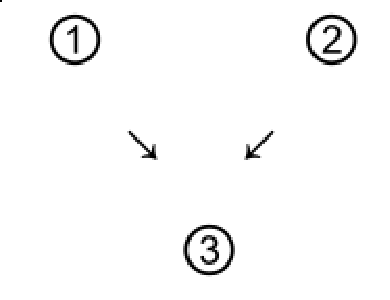
\includegraphics[scale=.49]{diagram1.pdf}
%%%%%%%%%%%
%%%%%%%%%%% pg 19 first one
%%%%%%%%%%%


\subsubsection{Intermediate Premises}
Some premises support their conclusions more directly than others. Premises provide more indirect
support for a conclusion by providing a reason to believe another premise that supports the
conclusion more directly. That is, some premises are intermediate between the conclusion and
other premises.

Consider this simple argument:

(1) Automatic weapons should be illegal. (2) They can be used to kill large numbers of
people in a short amount of time. This is because (3) all you have to do is hold down the
trigger and bullets come flying out in rapid succession.

The conclusion of this argument is the first proposition, so the premises are propositions 2 and 3.
Notice, though, that there's a relationship between those two claims. The third sentence starts with
the phrase `This is because', indicating that it provides a reason for another claim. The other claim
is proposition 2; `This' refers to the claim that automatic weapons can kill large numbers of people
quickly. Why should I believe that they can do that? Because all one has to do is hold down the
trigger to release lots of bullets really fast. Proposition 2 provides immediate support for the
conclusion (automatic weapons can kill lots of people really quickly, so we should make them
illegal); proposition 3 supports the conclusion more indirectly, by giving support to proposition 2.
Here is how we diagram in this case: \\

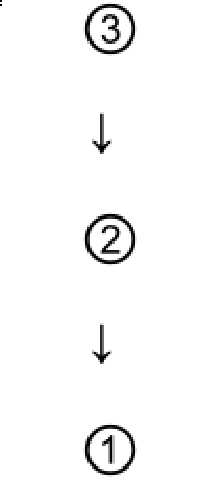
\includegraphics[scale=.49]{diagram2.pdf}
%%%%%%%%%%%%%%%
%%%%%%%%%%%%%%% pg 19 second one
%%%%%%%%%%%%%%%


\subsubsection{Joint Premises}
Sometimes premises need each other: the job of supporting another proposition can't be done by
each on its own; they can only provide support together, jointly. Far from being independent, such
premises are interdependent. In this situation, on our diagrams, we join together the interdependent
premises with a bracket underneath their circled numbers.

There are a number of different ways in which premises can provide joint support. Sometimes,
premises just fit together like a hand in a glove; or, switching metaphors, one premise is like the
key that fits into the other to unlock the proposition they jointly support. An example can make
this clear:

\begin{quote}
(1) The chef has decided that either salmon or chicken will be tonight's special. (2) Salmon
won't be the special. Therefore, (3) the special will be chicken.
\end{quote}

Neither premise 1 nor premise 2 can support the conclusion on its own. A useful rule of thumb for
checking whether one proposition can support another is this: read the first proposition, then say
the word `therefore', then read the second proposition; if it doesn't make any sense, then you can't
draw an arrow from the one to the other. Let's try it here: ``The chef has decided that either salmon
or chicken will be tonight's special; therefore, the special will be chicken.'' That doesn't make any
sense. What happened to salmon? Proposition 1 can't support the conclusion on its own. Neither
can the second: ``Salmon won't be the special; therefore, the special will be chicken.'' Again, that
makes no sense. Why chicken? What about steak, or lobster? The second proposition can't support
the conclusion on its own, either; it needs help from the first proposition, which tells us that if it's
not salmon, it's chicken. Propositions 1 and 2 need each other; they support the conclusion jointly.
This is how we diagram the argument: \\

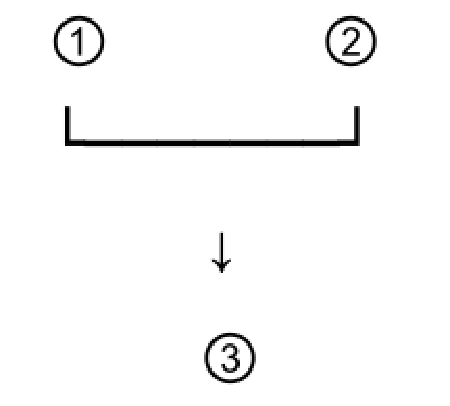
\includegraphics[scale=.49]{diagram3.pdf}
%%%%%%%%%%%%%%%%%%%
%%%%%%%%%%%%%%%%%%% page 20
%%%%%%%%%%%%%%%%%%%

The same diagram would depict the following argument:

\begin{quote}
(1) John Le Carre gives us realistic, three-dimensional characters and complex, interesting
plots. (2) Ian Fleming, on the other hand, presents an unrealistically glamorous picture of
international espionage, and his plotting isn't what you'd call immersive. (3) Le Carre is a
better author of spy novels than Fleming.
\end{quote}

In this example, the premises work jointly in a different way than in the previous example. Rather
than fitting together hand-in-glove, these premises each give us half of what we need to arrive at
the conclusion. The conclusion is a comparison between two authors. Each of the premises makes
claims about one of the two authors. Neither one, on its own, can support the comparison, because
the comparison is a claim about both of them. The premises can only support the conclusion
together. We would diagram this argument the same way as the last one.

Another common pattern for joint premises is when general propositions need help to provide
support for particular propositions. Consider the following argument:

(1) People shouldn't vote for racist, incompetent candidates for president. (2) Donald Trump
seems to make a new racist remark at least twice a week. And (3) he lacks the competence
to run even his own (failed) businesses, let alone the whole country. (4) You shouldn't vote
for Trump to be the president.

The conclusion of the argument, the thing it's trying to convince us of, is the last proposition--
you shouldn't vote for Trump. This is a particular claim: it's a claim about an individual person,
Trump. The first proposition in the argument, on the other hand, is a general claim: it asserts that,
generally speaking, people shouldn't vote for incompetent racists; it makes no mention of an
individual candidate. It cannot, therefore, support the particular conclusion--about Trump--on its
own. It needs help from other particular claims--propositions 2 and 3--that tell us that the
individual in the conclusion, Trump, meets the conditions laid out in the general proposition 1:
racism and incompetence. This is how we diagram the argument: \\

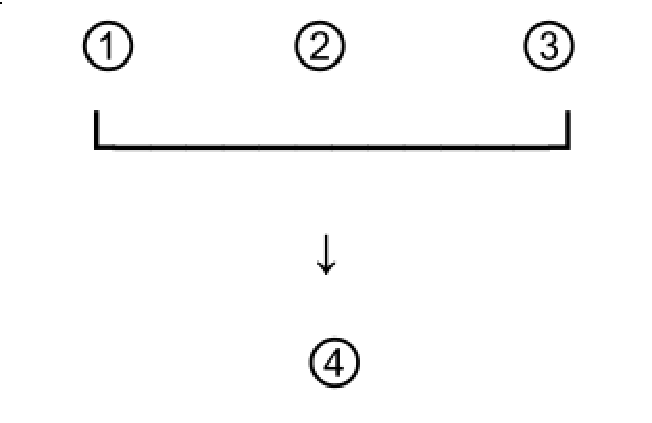
\includegraphics[scale=.49]{diagram4.pdf}
%%%%%%%%%%%%%%%
%%%%%%%%%%%%%%% pg 21
%%%%%%%%%%%%%%%


Occasionally, an argumentative passage will only explicitly state one of a set of joint premises
because the others ``go without saying''--they are part of the body of background information
about which both speaker and audience agree. In the last example, that Trump was an incompetent
racist was not uncontroversial background information. But consider this argument:

\begin{quote}
(1) It would be good for the country to have a woman with lots of experience in public
office as president. (2) People should vote for Hillary Clinton.
\end{quote}

Diagramming this argument seems straightforward: an arrow pointing from (1) to (2) But we've
got the same relationship between the premise and conclusion as in the last example: the premise
is a general claim, mentioning no individual at all, while the conclusion is a particular claim about
Hillary Clinton. Doesn't the general premise ``need help'' from particular claims to the effect that
the individual in question, Hillary Clinton, meets the conditions set forth in the premise--i.e., that
she's a woman and that she has lots of experience in public office? No, not really. Everybody
knows those things about her already; they go without saying, and can therefore be left unstated
(implicit, tacit).

But suppose we had included those obvious truths about Clinton in our presentation of the
argument; suppose we had made the tacit premises explicit:

\begin{quote}
(1) It would be good for the country to have a woman with lots of experience in public
office as president. (2) Hillary Clinton is a woman. And (3) she has deep experience with
public offices--as a First Lady, U.S. Senator, and Secretary of State. (4) People should vote
for Hillary Clinton.
\end{quote}

How do we diagram this? Earlier, we talked about a rule of thumb for determining whether or not
it's a good idea to draw an arrow from one number to another in a diagram: read the sentence
corresponding to the first number, say the word `therefore', then read the sentence corresponding
to the second number; if it doesn't make sense, then the arrow is a bad idea. But if it does make
sense, does that mean you should draw the arrow? Not necessarily. Consider the first and last
sentences in this passage. Read the first, then `therefore', then the last. Makes pretty good sense!
That's just the original formulation of the argument with the tacit propositions remaining implicit.
And in that case we said it would be OK to draw an arrow from the general premise's number
straight to the conclusion's. But when we add the tacit premises--the second and third sentences
in this passage--we can't draw an arrow directly from (1) to (4) To do so would obscure the
relationship among the first three propositions and misrepresent how the argument works. If we
drew an arrow from (1) to (4) what would we do with (2) to (3) in our diagram? Do they get their
own arrows, too? No, that won't do. Such a diagram would be telling us that the first three
propositions each independently provide a reason for the conclusion. But they're clearly not
independent; there's a relationship among them that our diagram must capture, and it's the same
relationship we saw in the parallel argument about Trump, with the particular claims in the second
and third propositions working together with the general claim in the first: \\


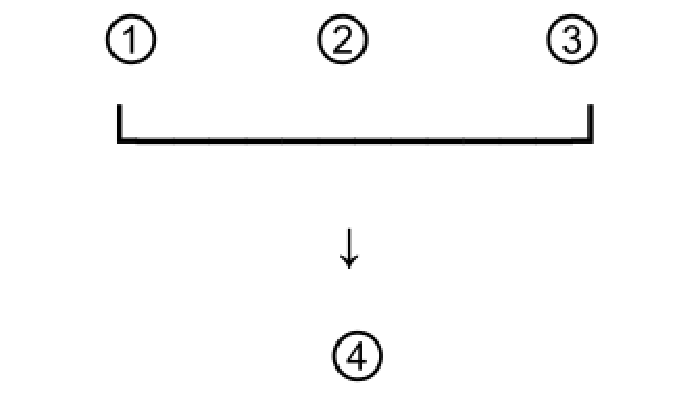
\includegraphics[scale=.49]{diagram5.pdf}
%%%%%%%%%%%%%%%
%%%%%%%%%%%%%%% same as on 21
%%%%%%%%%%%%%%%

The arguments we've looked at thus far have been quite short--only two or three premises. But of
course some arguments are longer than that. Some are much longer. The system of mapping generalizes 
to these longer arguments. In future lessons, we'll start to look at arguments with more and more 
premises.


EXERCISES \\

Diagram the following arguments.

\begin{enumerate}
\item (1) Hillary Clinton would make a better president than Donald Trump. (2) Clinton is a toughminded pragmatist who gets things done. (3) Trump is a thin-skinned maniac who will be totally
ineffective in dealing with Congress.

\item (1) Donald Trump is a jerk who's always offending people. Furthermore, (2) he has no
experience whatsoever in government. (3) Nobody should vote for him to be president.

\item (1) Human beings evolved to eat meat, so (2) eating meat is not immoral. (3) It's never immoral
for a creature to act according to its evolutionary instincts.

\item (1) We need new campaign finance laws in this country. (2) The influence of Wall Street money
on elections is causing a breakdown in our democracy with bad consequences for social justice.
(3) Politicians who have taken those donations are effectively bought and paid for, consistently
favoring policies that benefit the rich at the expense of the vast majority of citizens.

\item (1) Voters shouldn't trust any politician who took money from Wall Street bankers. (2) Hillary
Clinton accepted hundreds of thousands of dollars in speaking fee from Goldman Sachs, a big
Wall Street firm. (3) You shouldn't trust her.

\item (1) There are only three possible explanations for the presence of the gun at the crime scene:
either the defendant just happened to hide from the police right next to where the gun was found,
or the police planted the gun there after the fact, or it was really the defendant's gun like the
prosecution says. (2) The first option is too crazy a coincidence to be at all believable, and (3) we've
been given no evidence at all that the officers on the scene had any means or motivation to plant
the weapon. Therefore, (4) it has to be the defendant's gun.

\item (1) Golden State has to be considered the clear favorite to win the NBA Championship. (2) No
team has ever lost in the Finals after taking a 3-games-to-1 lead, and (3) Golden State now leads
Cleveland 3-to-1. In addition, (4) Golden State has the MVP of the league, Stephen Curry.

\item (1) We should increase funding to public colleges and universities. First of all, (2) as funding
has decreased, students have had to shoulder a larger share of the financial burden of attending
college, amassing huge amounts of debt. (3) A recent report shows that the average college student
graduates with almost \$30,000 in debt. Second, (4) funding public universities is a good
investment. (5) Every economist agrees that spending on public colleges is a good investment for
states, where the economic benefits far outweigh the amount spent.

\item (1) LED lightbulbs last for a really long time and (2) they cost very little to keep lit. (3) They
are, therefore, a great way to save money. (4) Old-fashioned incandescent bulbs, on the other hand,
are wasteful. (5) You should buy LEDs instead of incandescent bulbs.

\item (1) There's a hole in my left shoe, which means (2) my feet will get wet when I wear them in
the rain, and so (3) I'll probably catch a cold or something if I don't get a new pair of shoes.
Furthermore, (4) having new shoes would make me look cool. (5) I should buy new shoes.

\item Look, it's just simple economics: (1) if people stop buying a product, then companies will stop
producing it. And (2) people just aren't buying tablets as much anymore. (3) The CEO of Best Buy
recently said that sales of tablets are ``crashing'' at his stores. (4) Samsung's sales of tablets were
down 14\% 
this year alone. (5) Apple's not going to continue to make your beloved iPad for much
longer.

\item (1) We should increase infrastructure spending as soon as possible. Why? First, (2) the longer
we delay needed repairs to things like roads and bridges, the more they will cost in the future.
Second, (3) it would cause a drop in unemployment, as workers would be hired to do the work.
Third, (4) with interest rates at all-time lows, financing the spending would cost relatively little. A
fourth reason? (5) Economic growth. (6) Most economists agree that government spending in the
current climate would boost GDP.

\item  (1) Smoking causes cancer and (2) cigarettes are really expensive. (3) You should quit smoking.
(4) If you don't, you'll never get a girlfriend. (5) Smoking makes you less attractive to girls: (6) it
stains your teeth and (7) it gives you bad breath.
\end{enumerate}
